\documentclass[xcolor=svgnames]{beamer}\usepackage[]{graphicx}\usepackage[]{color}
%% maxwidth is the original width if it is less than linewidth
%% otherwise use linewidth (to make sure the graphics do not exceed the margin)
\makeatletter
\def\maxwidth{ %
  \ifdim\Gin@nat@width>\linewidth
    \linewidth
  \else
    \Gin@nat@width
  \fi
}
\makeatother

\definecolor{fgcolor}{rgb}{0.345, 0.345, 0.345}
\newcommand{\hlnum}[1]{\textcolor[rgb]{0.686,0.059,0.569}{#1}}%
\newcommand{\hlstr}[1]{\textcolor[rgb]{0.192,0.494,0.8}{#1}}%
\newcommand{\hlcom}[1]{\textcolor[rgb]{0.678,0.584,0.686}{\textit{#1}}}%
\newcommand{\hlopt}[1]{\textcolor[rgb]{0,0,0}{#1}}%
\newcommand{\hlstd}[1]{\textcolor[rgb]{0.345,0.345,0.345}{#1}}%
\newcommand{\hlkwa}[1]{\textcolor[rgb]{0.161,0.373,0.58}{\textbf{#1}}}%
\newcommand{\hlkwb}[1]{\textcolor[rgb]{0.69,0.353,0.396}{#1}}%
\newcommand{\hlkwc}[1]{\textcolor[rgb]{0.333,0.667,0.333}{#1}}%
\newcommand{\hlkwd}[1]{\textcolor[rgb]{0.737,0.353,0.396}{\textbf{#1}}}%

\usepackage{framed}
\makeatletter
\newenvironment{kframe}{%
 \def\at@end@of@kframe{}%
 \ifinner\ifhmode%
  \def\at@end@of@kframe{\end{minipage}}%
  \begin{minipage}{\columnwidth}%
 \fi\fi%
 \def\FrameCommand##1{\hskip\@totalleftmargin \hskip-\fboxsep
 \colorbox{shadecolor}{##1}\hskip-\fboxsep
     % There is no \\@totalrightmargin, so:
     \hskip-\linewidth \hskip-\@totalleftmargin \hskip\columnwidth}%
 \MakeFramed {\advance\hsize-\width
   \@totalleftmargin\z@ \linewidth\hsize
   \@setminipage}}%
 {\par\unskip\endMakeFramed%
 \at@end@of@kframe}
\makeatother

\definecolor{shadecolor}{rgb}{.97, .97, .97}
\definecolor{messagecolor}{rgb}{0, 0, 0}
\definecolor{warningcolor}{rgb}{1, 0, 1}
\definecolor{errorcolor}{rgb}{1, 0, 0}
\newenvironment{knitrout}{}{} % an empty environment to be redefined in TeX

\usepackage{alltt}
\usetheme{Boadilla}
\usecolortheme[named=SeaGreen]{structure}
\usepackage{graphicx}
\usepackage{breqn}
\usepackage{xcolor}
\usepackage{booktabs}
\usepackage{verbatim}
\usepackage{tikz}
\usepackage{lmodern}
\usetikzlibrary{shadows,arrows,positioning}
\definecolor{links}{HTML}{2A1B81}
\hypersetup{colorlinks,linkcolor=links,urlcolor=links}
\usepackage{pgfpages}

\newcommand{\Bigtxt}[1]{\textbf{\textit{#1}}}
\IfFileExists{upquote.sty}{\usepackage{upquote}}{}
\begin{document}

\title[Intro to EDA]{Introduction to exploratory data analysis}

\author[M. Beck, T. O'Brien]{Marcus W. Beck\inst{1} \and Todd D. O'Brien\inst{2}}

\date{}

\institute[]{\inst{1} ORISE, USEPA NHEERL Gulf Ecology Division\\ Email: \href{mailto:beck.marcus@epa.gov}{beck.marcus@epa.gov} \and \inst{2} NOAA/NMFS Copepod Project\\ Email: \href{todd.obrien@noaa.gov}{todd.obrien@noaa.gov}}

% knitr setup


% load SWMPr from local


%%%%%%
\begin{frame}
\vspace{0.3in}
\centerline{
\begin{tikzpicture}
  \node[drop shadow={shadow xshift=0ex,shadow yshift=0ex},fill=white,draw] at (0,0) {
\includegraphics[width=0.9\textwidth]{bg_main.jpg}};
\end{tikzpicture}}
\titlepage
\end{frame}

%%%%%%
\begin{frame}{Objectives and agenda}
\begin{itemize}
\onslide<+->
\item Objectives \\~\\
\begin{itemize}
\item What are some tools for pre-processing/organizing the SWMP data? \\~\\
\item What is the purpose of exploratory data analysis (EDA)? \\~\\
\item What are some common techniques and tools for EDA? \\~\\
\end{itemize}
\onslide<+->
\item Agenda \\~\\
\begin{itemize}
\item Review of data retrieval and import \\~\\
\item Organizing tools in SWMPr \\~\\
\item Purpose and overview of EDA \\~\\
\item Generic EDA tools in R, tools in SWMPr\\~\\
\end{itemize}
\end{itemize}
\end{frame}

%%%%%%
\begin{frame}{Interactive portion}
You can follow along in this module: \\~\\
\begin{itemize}
\item dataset2 \\~\\
\item script2 \\~\\
\end{itemize}
\Large
\centerline{\emph{Interactive! Interrupt me!}}
\end{frame}

%%%%%%
\begin{frame}{Retrieve SWMP data}
We learned how to import SWMP data in the previous session \\~\\
To review, the easiest approach is to download the data outside of R, then import using the `import_local' function \\~\\
Be sure that you use only the \href{http://cdmo.baruch.sc.edu/aqs/zips.cfm}{zip downloads} feature from CDMO - the `import_local' functions works best with these data \\~\\
\centerline{
\includegraphics[width = 0.8\textwidth]{adv_query.png}}
\end{frame}

%%%%%%
\begin{frame}[t]{Retrieve SWMP data}
We have provided data for use with the workshop\\~\\
For future access, it may be best to download all the data possible for a reserve to avoid repeated requests to the server and to centralize the location from which the data are imported into R \\~\\
\centerline{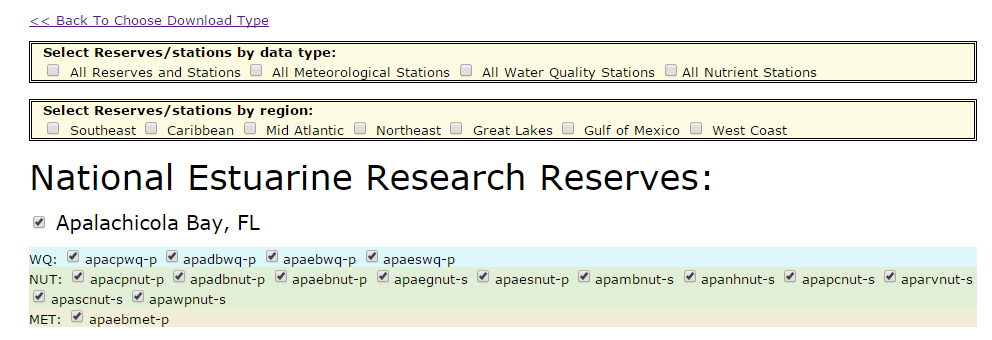
\includegraphics[width = \textwidth]{zip_eda.png}}
\end{frame}

%%%%%%
\begin{frame}[t]{Retrieve SWMP data}
It may be best to download all the data possible for a reserve to avoid repeated requests to the server and to centralize the location from which the data are imported into R \\~\\
\centerline{
\includegraphics[width = 0.5\textwidth]{zip_eda2.png}}
Here we've made a request for all stations at Apalachicola Bay (water quality, nutrients, weather) and all available years (1995--2014) \\~\\
This request will take several minutes to be delivered to your email - the files in `dataset2' are an abbreviate version of these data for this training module
\end{frame}

%%%%%%
\begin{frame}[containsverbatim]{Retrieve SWMP data}
Let's import some data for Apalachicola Bay

\begin{knitrout}\scriptsize
\definecolor{shadecolor}{rgb}{0.969, 0.969, 0.969}\color{fgcolor}\begin{kframe}
\begin{alltt}
\hlcom{# reload the SWMPr package if you started a new session}
\hlkwd{library}\hlstd{(SWMPr)}

\hlcom{# import data}
\hlcom{# change this path for the flash drive}
\hlstd{path} \hlkwb{<-} \hlstr{'C:/data/dataset2'}
\hlstd{wq_dat} \hlkwb{<-} \hlkwd{import_local}\hlstd{(path,} \hlstr{'apacpwq'}\hlstd{)}
\hlstd{nut_dat} \hlkwb{<-} \hlkwd{import_local}\hlstd{(path,} \hlstr{'apacpnut'}\hlstd{)}
\hlstd{met_dat} \hlkwb{<-} \hlkwd{import_local}\hlstd{(path,} \hlstr{'apaebmet'}\hlstd{)}
\end{alltt}
\end{kframe}
\end{knitrout}
We've just imported data from 2011--2014 for three stations (apacpwq, apacpnut, apaebmet) and saved them in our workspace as three separate objects (wq\_dat, nut\_dat, met\_dat)
\end{frame}

%%%%%%
\begin{frame}[containsverbatim]{Retrieve SWMP data}
But don't take my word for it, take a look at the data!
\begin{knitrout}\scriptsize
\definecolor{shadecolor}{rgb}{0.969, 0.969, 0.969}\color{fgcolor}\begin{kframe}
\begin{alltt}
\hlcom{# what are the dimenions of the water quality data?}
\hlkwd{dim}\hlstd{(wq_dat)}
\end{alltt}
\begin{verbatim}
## [1] 132035     25
\end{verbatim}
\begin{alltt}
\hlcom{# what are the dimenions of the nutrient data?}
\hlkwd{dim}\hlstd{(nut_dat)}
\end{alltt}
\begin{verbatim}
## [1] 48 13
\end{verbatim}
\begin{alltt}
\hlcom{# what are the dimenions of the weather data?}
\hlkwd{dim}\hlstd{(met_dat)}
\end{alltt}
\begin{verbatim}
## [1] 133548     23
\end{verbatim}
\end{kframe}
\end{knitrout}
\end{frame}

%%%%%%
\begin{frame}[containsverbatim,shrink]{Retrieve SWMP data}
View the first six rows
\begin{knitrout}\scriptsize
\definecolor{shadecolor}{rgb}{0.969, 0.969, 0.969}\color{fgcolor}\begin{kframe}
\begin{alltt}
\hlcom{# View the first six rows of the wq data}
\hlkwd{head}\hlstd{(met_dat)}
\end{alltt}
\begin{verbatim}
##         datetimestamp atemp f_atemp rh f_rh   bp f_bp wspd f_wspd maxwspd
## 1 2011-01-01 00:00:00    15    <0>  94 <0>  1019 <0>     3   <0>        3
## 2 2011-01-01 00:15:00    15    <0>  95 <0>  1019 <0>     3   <0>        4
## 3 2011-01-01 00:30:00    15    <0>  95 <0>  1019 <0>     3   <0>        4
## 4 2011-01-01 00:45:00    15    <0>  95 <0>  1019 <0>     3   <0>        4
## 5 2011-01-01 01:00:00    15    <0>  95 <0>  1018 <0>     3   <0>        4
## 6 2011-01-01 01:15:00    15    <0>  95 <0>  1018 <0>     4   <0>        5
##   f_maxwspd wdir f_wdir sdwdir f_sdwdir totpar  f_totpar totprcp f_totprcp
## 1      <0>   145   <0>       8     <0>     0.8 <1> (CSM)       0      <0> 
## 2      <0>   146   <0>       7     <0>     0.8 <1> (CSM)       0      <0> 
## 3      <0>   139   <0>       7     <0>     0.8 <1> (CSM)       0      <0> 
## 4      <0>   140   <0>       7     <0>     0.8 <1> (CSM)       0      <0> 
## 5      <0>   144   <0>       6     <0>     0.8 <1> (CSM)       0      <0> 
## 6      <0>   141   <0>       7     <0>     0.8 <1> (CSM)       0      <0> 
##   cumprcp f_cumprcp totsorad f_totsorad
## 1       0      <0>        NA      <-1> 
## 2       0      <0>        NA      <-1> 
## 3       0      <0>        NA      <-1> 
## 4       0      <0>        NA      <-1> 
## 5       0      <0>        NA      <-1> 
## 6       0      <0>        NA      <-1>
\end{verbatim}
\end{kframe}
\end{knitrout}
\end{frame}

%%%%%%
\begin{frame}[containsverbatim,shrink]{Retrieve SWMP data}
View the last six rows
\begin{knitrout}\scriptsize
\definecolor{shadecolor}{rgb}{0.969, 0.969, 0.969}\color{fgcolor}\begin{kframe}
\begin{alltt}
\hlcom{# View the last six rows of the wq data}
\hlkwd{tail}\hlstd{(met_dat)}
\end{alltt}
\begin{verbatim}
##              datetimestamp atemp f_atemp rh f_rh   bp f_bp wspd f_wspd maxwspd
## 133543 2014-10-23 01:30:00    14    <0>  72 <0>  1017 <0>     3   <0>        5
## 133544 2014-10-23 01:45:00    14    <0>  72 <0>  1016 <0>     3   <0>        5
## 133545 2014-10-23 02:00:00    14    <0>  74 <0>  1016 <0>     3   <0>        4
## 133546 2014-10-23 02:15:00    14    <0>  74 <0>  1016 <0>     3   <0>        4
## 133547 2014-10-23 02:30:00    14    <0>  75 <0>  1016 <0>     3   <0>        4
## 133548 2014-10-23 02:45:00    14    <0>  76 <0>  1016 <0>     2   <0>        4
##        f_maxwspd wdir f_wdir sdwdir f_sdwdir totpar f_totpar totprcp f_totprcp
## 133543      <0>    33   <0>       9     <0>       0     <0>        0      <0> 
## 133544      <0>    34   <0>      11     <0>       0     <0>        0      <0> 
## 133545      <0>    36   <0>      10     <0>       0     <0>        0      <0> 
## 133546      <0>    43   <0>      11     <0>       0     <0>        0      <0> 
## 133547      <0>    41   <0>      10     <0>       0     <0>        0      <0> 
## 133548      <0>    42   <0>      10     <0>       0     <0>        0      <0> 
##        cumprcp f_cumprcp totsorad f_totsorad
## 133543      NA     <-2>        NA      <-1> 
## 133544      NA     <-2>        NA      <-1> 
## 133545      NA     <-2>        NA      <-1> 
## 133546      NA     <-2>        NA      <-1> 
## 133547      NA     <-2>        NA      <-1> 
## 133548      NA     <-2>        NA      <-1>
\end{verbatim}
\end{kframe}
\end{knitrout}
\end{frame}

%%%%%%
\begin{frame}[containsverbatim,shrink]{Retrieve SWMP data}
We'll first work with the water quality records\\~\\
What class is the data?
\begin{knitrout}\scriptsize
\definecolor{shadecolor}{rgb}{0.969, 0.969, 0.969}\color{fgcolor}\begin{kframe}
\begin{alltt}
\hlcom{# class of the data}
\hlkwd{class}\hlstd{(met_dat)}
\end{alltt}
\begin{verbatim}
## [1] "swmpr"      "data.frame"
\end{verbatim}
\end{kframe}
\end{knitrout}
This tells us that the data are two different classes - `swmpr' and `data.frame'\\~\\
The class of an object is important because it defines the types of methods (i.e., functions) that apply\\~\\
For example, `head' and `tail' functions work for a `data.frame'
\end{frame}

%%%%%%
\begin{frame}[containsverbatim,shrink]{Retrieve SWMP data}
The swmpr object class was developed to make your life easier working with SWMP data\\~\\
The \href{https://github.com/fawda123/SWMPr}{online documentation} describes the functions that work with the swmpr object class, also...
\begin{knitrout}\scriptsize
\definecolor{shadecolor}{rgb}{0.969, 0.969, 0.969}\color{fgcolor}\begin{kframe}
\begin{alltt}
\hlcom{# what functions/methods work with swmpr objects?}
\hlkwd{methods}\hlstd{(}\hlkwc{class} \hlstd{=} \hlstr{'swmpr'}\hlstd{)}
\end{alltt}
\begin{verbatim}
##  [1] aggregate.swmpr comb.swmpr      decomp.swmpr    hist.swmpr     
##  [5] lines.swmpr     na.approx.swmpr plot.swmpr      qaqc.swmpr     
##  [9] qaqcchk.swmpr   setstep.swmpr   smoother.swmpr  subset.swmpr
\end{verbatim}
\end{kframe}
\end{knitrout}
Documentation of each function can be viewed as follows (although currently not complete):
\begin{knitrout}\scriptsize
\definecolor{shadecolor}{rgb}{0.969, 0.969, 0.969}\color{fgcolor}\begin{kframe}
\begin{alltt}
\hlcom{# see help for a swmpr function}
\hlopt{?}\hlstd{aggregate.swmpr}

\hlcom{# or...}
\hlkwd{help}\hlstd{(}\hlstr{'aggregate.swmpr'}\hlstd{)}
\end{alltt}
\end{kframe}
\end{knitrout}
\end{frame}

%%%%%%
\begin{frame}[containsverbatim,shrink]{Retrieve SWMP data}
A side note about R syntax... the convention `function.class' means that a function applies to a specific class \\~\\
The `function' is generic, whereas the `function.class' is a method for a class that applies to the generic
\begin{knitrout}\scriptsize
\definecolor{shadecolor}{rgb}{0.969, 0.969, 0.969}\color{fgcolor}\begin{kframe}
\begin{alltt}
\hlcom{# view the methods that apply to the generic aggregate}
\hlkwd{methods}\hlstd{(}\hlstr{'aggregate'}\hlstd{)}
\end{alltt}
\begin{verbatim}
## [1] aggregate.data.frame aggregate.default*   aggregate.formula*  
## [4] aggregate.swmpr      aggregate.ts         aggregate.zoo*      
## 
##    Non-visible functions are asterisked
\end{verbatim}
\end{kframe}
\end{knitrout}
A function with a class method can be executed using shorthand...
\begin{knitrout}\scriptsize
\definecolor{shadecolor}{rgb}{0.969, 0.969, 0.969}\color{fgcolor}\begin{kframe}
\begin{alltt}
\hlcom{# shorthand for executing aggregate on a swmpr object}
\hlkwd{aggregate}\hlstd{(met_dat,} \hlkwc{by} \hlstd{=} \hlstr{'quarters'}\hlstd{)}

\hlcom{# long also works}
\hlkwd{aggregate.swmpr}\hlstd{(met_dat,} \hlkwc{by} \hlstd{=} \hlstr{'quarters'}\hlstd{)}
\end{alltt}
\end{kframe}
\end{knitrout}
\end{frame}

%%%%%
\begin{frame}[containsverbatim,shrink]{Retrieve SWMP data}
A useful feature of R is that a class will have both \Bigtxt{data} and \Bigtxt{attributes}\\~\\
For the swmpr class, the \Bigtxt{data} are the raw swmpr data as a data.frame \\~\\
The \Bigtxt{attributes} are a list of metadata for the imported data
\begin{knitrout}\scriptsize
\definecolor{shadecolor}{rgb}{0.969, 0.969, 0.969}\color{fgcolor}\begin{kframe}
\begin{alltt}
\hlcom{# what attributes are available for a swmpr object}
\hlkwd{names}\hlstd{(}\hlkwd{attributes}\hlstd{(met_dat))}
\end{alltt}
\begin{verbatim}
## [1] "names"       "row.names"   "class"       "station"     "parameters" 
## [6] "qaqc_cols"   "date_rng"    "timezone"    "stamp_class"
\end{verbatim}
\begin{alltt}
\hlcom{# view the parameters}
\hlkwd{attr}\hlstd{(met_dat,} \hlstr{'parameters'}\hlstd{)}
\end{alltt}
\begin{verbatim}
##  [1] "atemp"    "rh"       "bp"       "wspd"     "maxwspd"  "wdir"    
##  [7] "sdwdir"   "totpar"   "totprcp"  "cumprcp"  "totsorad"
\end{verbatim}
\end{kframe}
\end{knitrout}
\end{frame}

%%%%%
\begin{frame}[containsverbatim]{Retrieve SWMP data}
You can also view all the attributes as follows:
\begin{knitrout}\scriptsize
\definecolor{shadecolor}{rgb}{0.969, 0.969, 0.969}\color{fgcolor}\begin{kframe}
\begin{alltt}
\hlcom{# view all attributes}
\hlkwd{attributes}\hlstd{(met_dat)}
\end{alltt}
\end{kframe}
\end{knitrout}
This is not recommended since they are quite long, e.g., an attribute of the `data.frame' class is the row names (132035 rows for`wq\_dat') \\~\\
Individual attributes are useful for getting a feel for the dataset - what is the date range? what parameters are included? are QAQC columns present? \\~\\
However, the intended use of attributes is behind the scenes with swmpr functions - they will be used to process the data and updated automatically
\end{frame}

%%%%%%
\begin{frame}[containsverbatim]{Retrieve SWMP data}
A summary of the swmpr object class:\\~\\
\begin{itemize}
\item Throughout `SWMPr' refers to the \Bigtxt{package}, `swmpr' refers to the object \Bigtxt{class}
\item \Bigtxt{Methods} aka functions in the SWMPr package are specific for swmpr objects - see the help documentation (`?aggregate.swmpr')
\item The swmpr object has both \Bigtxt{data} and \Bigtxt{attributes} - the data are in the `data.frame' format, the attributes are in a `list'\\~\\
\end{itemize}
These are basic concepts that are fundamental to how the R language works -- you should have a general understanding of their meaning
\end{frame}

%%%%%%
\begin{frame}[containsverbatim,shrink]{Organize SWMP data}
Now that we have a feel for the data, what needs to be done before we can start analyzing the information? \\~\\
Last module: \\~\\
\begin{itemize}
\item How do we handle QAQC data or `bad' observations?
\item How do we deal with data we don't want?  
\item How do we combine data for comparison?
\item How do we handle issues inherent with time series? \\~\\
\end{itemize}
Several of these problems are context-dependent - driven by the question or analysis \\~\\
Others are common to any analysis...
\end{frame}

%%%%%%
\begin{frame}[containsverbatim]{Organize SWMP data}
Perhaps the first organizational tool you want to use is `qaqc.swmpr'\\~\\
This function does two things:\\~\\
\begin{itemize}
\item Remove observations with a specified QAQC flag value
\item Remove extraneous QAQC columns \\~\\
\end{itemize}
\centerline{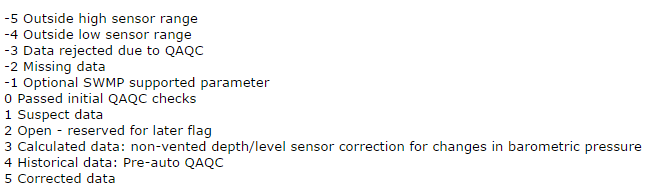
\includegraphics[width = 0.8\textwidth]{qaqc_flags.png}}
\end{frame}

%%%%%%
\begin{frame}[containsverbatim]{Organize SWMP data}
You will have to decide which \href{http://cdmo.baruch.sc.edu/data/qaqc.cfm}{values} to keep - be conservative and only keep those that passed QAQC or keep all the data \\~\\
To help you decide, it may be useful to get an idea of the distribution of QAQC flags in the data
\begin{knitrout}\scriptsize
\definecolor{shadecolor}{rgb}{0.969, 0.969, 0.969}\color{fgcolor}\begin{kframe}
\begin{alltt}
\hlcom{# use qaqcchk to view distribution of qaqc flags}
\hlstd{myqaqc} \hlkwb{<-} \hlkwd{qaqcchk}\hlstd{(met_dat)}
\end{alltt}
\end{kframe}
\end{knitrout}
This function returns a data.frame\\~\\
\begin{itemize}
\item The first column shows all the QAQC codes in the data
\item The remaining columns show the counts for each parameter of the observations assigned to each QAQC code
\end{itemize}
\end{frame}

%%%%%%
\begin{frame}[containsverbatim]{Organize SWMP data}
\begin{knitrout}\scriptsize
\definecolor{shadecolor}{rgb}{0.969, 0.969, 0.969}\color{fgcolor}\begin{kframe}
\begin{alltt}
\hlcom{# a subset of results from the qaqcchk function}
\hlkwd{head}\hlstd{(myqaqc)}
\end{alltt}
\begin{verbatim}
##              piece f_atemp f_bp f_cumprcp f_maxwspd f_rh f_sdwdir f_totpar
## 1       <-2> [GPD]       2    2         2         2    2        2        2
## 2       <-3> [GMT]       5   13        70        16    5       16       18
## 3       <-3> [GPD]      15   16        16        16   15       16       16
## 4       <-3> [GPR]      14   14        14        14   14       14       13
## 5       <-3> [SMT]       2   NA       121         3    2        3        2
## 6 <-3> [SQR] (CSM)       3   NA        NA        NA    3       NA     4023
##   f_totprcp f_totsorad f_wdir f_wspd
## 1         2         NA      2      2
## 2        13         NA     16     16
## 3        16         NA     16     16
## 4        14         NA     14     14
## 5        14         NA      3      3
## 6        NA         NA     NA     NA
\end{verbatim}
\begin{alltt}
\hlcom{# or view all in a separate window}
\hlkwd{View}\hlstd{(myqaqc)}
\end{alltt}
\end{kframe}
\end{knitrout}
\href{http://cdmo.baruch.sc.edu/data/qaqc.cfm}{Link} to QAQC codes
\end{frame}

%%%%%%
\begin{frame}[containsverbatim]{Organize SWMP data}
A plot of the data can be useful to view QAQC flags, but this is tedious
\begin{knitrout}\scriptsize
\definecolor{shadecolor}{rgb}{0.969, 0.969, 0.969}\color{fgcolor}\begin{kframe}
\begin{alltt}
\hlcom{# select values that did not pass qaqc}
\hlstd{nopass} \hlkwb{<-} \hlkwd{grep}\hlstd{(}\hlstr{'0'}\hlstd{, met_dat}\hlopt{$}\hlstd{f_totpar,} \hlkwc{invert} \hlstd{= T)}
\hlstd{nopass} \hlkwb{<-} \hlstd{met_dat[nopass, ]}

\hlcom{# plot totpar from met_dat}
\hlkwd{plot}\hlstd{(totpar} \hlopt{~} \hlstd{datetimestamp, met_dat,} \hlkwc{type} \hlstd{=} \hlstr{'l'}\hlstd{)}

\hlcom{# add  points that did not pass qaqc}
\hlkwd{points}\hlstd{(nopass}\hlopt{$}\hlstd{datetimestamp, nopass}\hlopt{$}\hlstd{totpar,} \hlkwc{col} \hlstd{=} \hlstr{'red'}\hlstd{)}
\end{alltt}
\end{kframe}
\end{knitrout}
\end{frame}

%%%%%%
\begin{frame}[containsverbatim]{Organize SWMP data}
A plot of the data can be useful to view QAQC flags, but this is tedious
\begin{knitrout}\scriptsize
\definecolor{shadecolor}{rgb}{0.969, 0.969, 0.969}\color{fgcolor}

{\centering 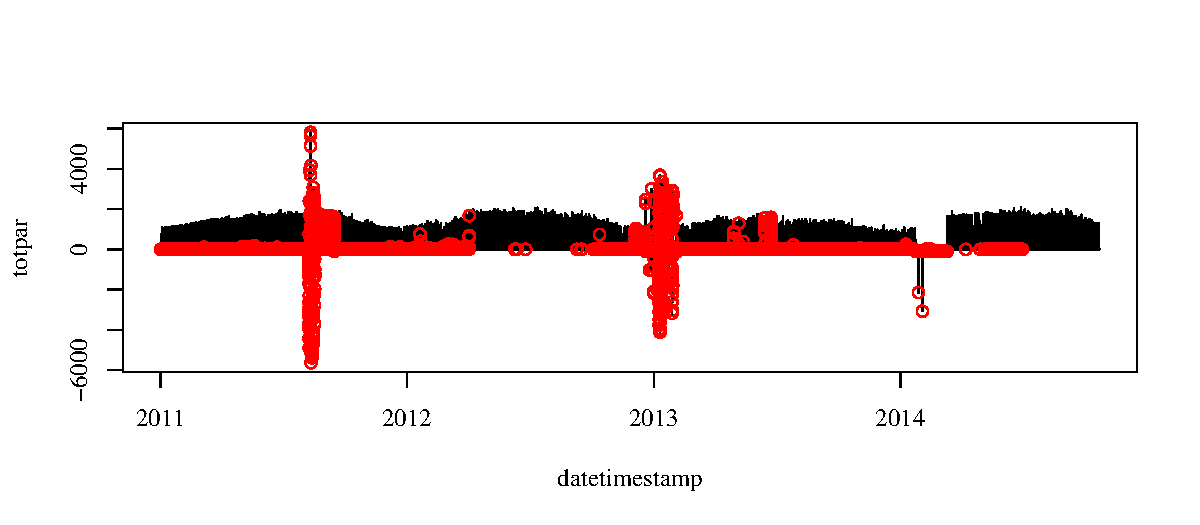
\includegraphics[width=\maxwidth]{figure/qaqc_ex} 

}



\end{knitrout}
Does this plot make sense??
\end{frame}

%%%%%%
\begin{frame}[containsverbatim]{Organize SWMP data}
You should have an idea of how you want to handle QAQC values after viewing the output from qaqcchk - or you already knew \\~\\
Next, use the qaqc function...
\begin{knitrout}\scriptsize
\definecolor{shadecolor}{rgb}{0.969, 0.969, 0.969}\color{fgcolor}\begin{kframe}
\begin{alltt}
\hlcom{# filter observations by qaqc flags, remove qaqc columns}
\hlstd{met_qaqc} \hlkwb{<-} \hlkwd{qaqc}\hlstd{(met_dat)}
\end{alltt}
\end{kframe}
\end{knitrout}
The default behavior for this function is to keep only observations with a `0' QAQC flag - data that passed initial checks\\~\\
See the help documentation for the function
\begin{knitrout}\scriptsize
\definecolor{shadecolor}{rgb}{0.969, 0.969, 0.969}\color{fgcolor}\begin{kframe}
\begin{alltt}
\hlcom{# view help file}
\hlopt{?}\hlstd{qaqc}
\end{alltt}
\end{kframe}
\end{knitrout}
\end{frame}

%%%%%%
\begin{frame}[containsverbatim]{Organize SWMP data}
View the data after keeping only values that passed QAQC (`0' flag)
\begin{knitrout}\scriptsize
\definecolor{shadecolor}{rgb}{0.969, 0.969, 0.969}\color{fgcolor}\begin{kframe}
\begin{alltt}
\hlcom{# data after qaqc processing}
\hlkwd{head}\hlstd{(met_qaqc)}
\end{alltt}
\begin{verbatim}
##         datetimestamp atemp rh   bp wspd maxwspd wdir sdwdir totpar totprcp
## 1 2011-01-01 00:00:00    15 94 1019    3       3  145      8     NA       0
## 2 2011-01-01 00:15:00    15 95 1019    3       4  146      7     NA       0
## 3 2011-01-01 00:30:00    15 95 1019    3       4  139      7     NA       0
## 4 2011-01-01 00:45:00    15 95 1019    3       4  140      7     NA       0
## 5 2011-01-01 01:00:00    15 95 1018    3       4  144      6     NA       0
## 6 2011-01-01 01:15:00    15 95 1018    4       5  141      7     NA       0
##   cumprcp totsorad
## 1       0       NA
## 2       0       NA
## 3       0       NA
## 4       0       NA
## 5       0       NA
## 6       0       NA
\end{verbatim}
\end{kframe}
\end{knitrout}
\end{frame}

%%%%%%
\begin{frame}[containsverbatim]{Organize SWMP data}
What if we want to keep all the values, regardless of flag?
\begin{knitrout}\scriptsize
\definecolor{shadecolor}{rgb}{0.969, 0.969, 0.969}\color{fgcolor}\begin{kframe}
\begin{alltt}
\hlcom{# keep all values}
\hlstd{met_qaqc} \hlkwb{<-} \hlkwd{qaqc}\hlstd{(met_dat,} \hlkwc{qaqc_keep} \hlstd{=} \hlkwa{NULL}\hlstd{)}

\hlkwd{head}\hlstd{(met_qaqc)} \hlcom{# note the totpar column compared to the last example}
\end{alltt}
\begin{verbatim}
##         datetimestamp atemp rh   bp wspd maxwspd wdir sdwdir totpar totprcp
## 1 2011-01-01 00:00:00    15 94 1019    3       3  145      8    0.8       0
## 2 2011-01-01 00:15:00    15 95 1019    3       4  146      7    0.8       0
## 3 2011-01-01 00:30:00    15 95 1019    3       4  139      7    0.8       0
## 4 2011-01-01 00:45:00    15 95 1019    3       4  140      7    0.8       0
## 5 2011-01-01 01:00:00    15 95 1018    3       4  144      6    0.8       0
## 6 2011-01-01 01:15:00    15 95 1018    4       5  141      7    0.8       0
##   cumprcp totsorad
## 1       0       NA
## 2       0       NA
## 3       0       NA
## 4       0       NA
## 5       0       NA
## 6       0       NA
\end{verbatim}
\end{kframe}
\end{knitrout}
\end{frame}

%%%%%%
\begin{frame}[containsverbatim]{Organize SWMP data}
If you're not convinced, try removing only the `0' flag
\begin{knitrout}\scriptsize
\definecolor{shadecolor}{rgb}{0.969, 0.969, 0.969}\color{fgcolor}\begin{kframe}
\begin{alltt}
\hlcom{# keep all values}
\hlstd{to_keep} \hlkwb{<-} \hlkwd{c}\hlstd{(}\hlopt{-}\hlnum{5}\hlstd{,} \hlopt{-}\hlnum{4}\hlstd{,} \hlopt{-}\hlnum{3}\hlstd{,} \hlopt{-}\hlnum{2}\hlstd{,} \hlopt{-}\hlnum{1}\hlstd{,} \hlnum{1}\hlstd{,} \hlnum{2}\hlstd{,} \hlnum{3}\hlstd{,} \hlnum{4}\hlstd{,} \hlnum{5}\hlstd{)}
\hlstd{met_qaqc} \hlkwb{<-} \hlkwd{qaqc}\hlstd{(met_dat,} \hlkwc{qaqc_keep} \hlstd{= to_keep)}

\hlcom{# does this result make sense??}
\hlkwd{head}\hlstd{(met_qaqc)}
\end{alltt}
\begin{verbatim}
##         datetimestamp atemp rh bp wspd maxwspd wdir sdwdir totpar totprcp
## 1 2011-01-01 00:00:00    NA NA NA   NA      NA   NA     NA    0.8      NA
## 2 2011-01-01 00:15:00    NA NA NA   NA      NA   NA     NA    0.8      NA
## 3 2011-01-01 00:30:00    NA NA NA   NA      NA   NA     NA    0.8      NA
## 4 2011-01-01 00:45:00    NA NA NA   NA      NA   NA     NA    0.8      NA
## 5 2011-01-01 01:00:00    NA NA NA   NA      NA   NA     NA    0.8      NA
## 6 2011-01-01 01:15:00    NA NA NA   NA      NA   NA     NA    0.8      NA
##   cumprcp totsorad
## 1      NA       NA
## 2      NA       NA
## 3      NA       NA
## 4      NA       NA
## 5      NA       NA
## 6      NA       NA
\end{verbatim}
\end{kframe}
\end{knitrout}
\end{frame}

%%%%%%
\begin{frame}[containsverbatim]{Organize SWMP data}
We'll continue by using values that passed the QAQC checks
\begin{knitrout}\scriptsize
\definecolor{shadecolor}{rgb}{0.969, 0.969, 0.969}\color{fgcolor}\begin{kframe}
\begin{alltt}
\hlcom{# continue with qaqc processed data}

\hlcom{# water quality}
\hlcom{# note the column number before/after qaqc processing}
\hlkwd{dim}\hlstd{(wq_dat)}
\end{alltt}
\begin{verbatim}
## [1] 132035     25
\end{verbatim}
\begin{alltt}
\hlstd{wq_dat} \hlkwb{<-} \hlkwd{qaqc}\hlstd{(wq_dat)}
\hlkwd{dim}\hlstd{(wq_dat)}
\end{alltt}
\begin{verbatim}
## [1] 132035     13
\end{verbatim}
\begin{alltt}
\hlcom{# nutrients}
\hlstd{nut_dat} \hlkwb{<-} \hlkwd{qaqc}\hlstd{(nut_dat)}

\hlcom{# weather}
\hlstd{met_dat} \hlkwb{<-} \hlkwd{qaqc}\hlstd{(met_dat)}
\end{alltt}
\end{kframe}
\end{knitrout}
\end{frame}

%%%%%%
\begin{frame}[containsverbatim]{Organize SWMP data}
What is the next logical step after dealing with QAQC values? \\~\\
How would we further want to organize the data? \\~\\
Maybe we want to subset the data... \\~\\
For example, we don't want all the data columns or we only want to work with a specific date range \\~\\
Use the subset function...
\begin{knitrout}\scriptsize
\definecolor{shadecolor}{rgb}{0.969, 0.969, 0.969}\color{fgcolor}\begin{kframe}
\begin{alltt}
\hlopt{?}\hlstd{subset.swmpr}
\end{alltt}
\end{kframe}
\end{knitrout}
Note that R has a generic subset function, subset.swmpr is a subset method for swmpr objects
\end{frame}

%%%%%%
\begin{frame}[containsverbatim]{Organize SWMP data}
The subset.swmpr function has several arguments
\begin{knitrout}\scriptsize
\definecolor{shadecolor}{rgb}{0.969, 0.969, 0.969}\color{fgcolor}\begin{kframe}
\begin{alltt}
\hlkwd{formals}\hlstd{(subset.swmpr)}
\end{alltt}
\begin{verbatim}
## $swmpr_in
## 
## 
## $subset
## NULL
## 
## $select
## NULL
## 
## $operator
## NULL
## 
## $rem_rows
## F
## 
## $rem_cols
## F
\end{verbatim}
\end{kframe}
\end{knitrout}
\end{frame}

% %%%%%%
% \begin{frame}[containsverbatim]{Organize SWMP data}
% 
% \end{frame}

%%%%%%
\begin{frame}
\vspace{0.3in}
\centerline{
\begin{tikzpicture}
  \node[drop shadow={shadow xshift=0ex,shadow yshift=0ex},fill=white,draw] at (0,0) {
\includegraphics[width=0.9\textwidth]{bg_main.jpg}};
\end{tikzpicture}}
\vspace{0.5in}
\Large
\centerline{\Bigtxt{Questions??}}
\end{frame}

\end{document}
